\documentclass[a4paper,10.0pt,twoside]{npr}

\usepackage{multicol,graphicx,lastpage,footmisc,fancyhdr,paralist,
tabularx,array,booktabs,caption,multirow,upgreek,mathrsfs,gensymb,color}
\usepackage[fancyhdr,space,fntef,fontset=ubuntu]{ctex}
\usepackage{amssymb,bm,mathrsfs,bbm,amscd}
\usepackage{flushend,cuted}
\usepackage{refcount}
\usepackage{savesym}
\usepackage{textcomp}
\usepackage[tbtags]{amsmath}  %
\savesymbol{iint}
\usepackage{amstext} %数学宏包文本命令
\usepackage{balance} %版心底部对齐

\flushbottom      %版心底部对齐
\setcounter{section}{0}
\begin{document}
%\begin{CJK*}{GBK}{\song}{\wuhao}{\rm}

%___________________________________________________________________________________
\def\rd{{\rm d}}

\newcommand{\RM}{\ensuremath{\mathrm}}   %正体 既可用于文本模式也可用于数学模式
\newcommand{\dif}{\mathrm{d}}  %直立体d
\newcommand{\me}{\mathrm{e}}  %直立体e
\newcommand{\mi}{\mathrm{i}}  %直立体i
\newcommand{\mj}{\mathrm{j}}  %直立体j
\newcommand{\afrac}[2]{\dfrac{\,#1\,}{\,#2\,}}  %略长分数线
\newcommand{\nn}{\nonumber}  %公式无编号
\newcommand{\nt}{\noindent}
\newcommand{\OO}{~\text{。}}
\newcommand{\PP}{~\text{,}}
\newcommand{\OP}{~\text{;}}
\newcommand{\LT}{\left}
\newcommand{\RT}{\right}

%___________________________________________________________________________________

\balance
\fancypagestyle{myfoot}
{%
\fancyhf{}
\fancyhead[c]{\wuhao\song 高~等~核~物~理~实~验}
\renewcommand{\headrule}{\vskip 2pt
\hrule height0.4pt width\headwidth \vskip1pt
\hrule height0.4pt width\headwidth \vskip-1.8pt}
}%
\thispagestyle{myfoot}

%%%%%%%%%%%%%%%%%%%%%%%%%%%%%%%%%%%%%%%%%%%%%%%%%%%%%
%    奇偶页眉
%%%%%%%%%%%%%%%%%%%%%%%%%%%%%%%%%%%%%%%%%%%%%%%%%%%%%
\pagestyle{fancy}
\fancyhead{}
\fancyhead[ce]{\xiaowu\song \hspace{0.5em}高~等~核~物~理~实~验}
%\fancyhead[ro,le]{\xiaowuhao \hspace{0.5em}\textbf{\textperiodcentered}\;\thepage\;\textbf{\textperiodcentered}\hspace{0.5em}}
%\fancyhead[ce]{\xiaowu\song 粒~子~物~理~与~原~子~核~物~理~专~题~实~验}
%\fancyhead[re]{\xiaowu\song \hspace{0.5em}第\;31\;卷\hspace{0.5em}}
\fancyfoot[ce,co]{}
\renewcommand{\headrule}{\vskip 2pt
\hrule height0.4pt width\headwidth}


\setcounter{page}{001}%
\fancyhead[co]{\xiaowuhao\song  乔颢:高纯锗$\gamma$射线谱仪}    %奇页页眉
\begin{center}
\title{%
\xiaoerhao \bf  %章标题为两行时改为 \exiaoer
高纯锗$\gamma$射线谱仪\\[-5mm]}
\maketitle
\large \fs
乔颢$^{^1}$\\[2mm]

\xiaowu \song
1. 北京大学物理学院,海淀区 北京 100871;\\[4mm]

 
\footnotetext[0]{{\bf 作者简介:}~~\begin{minipage}[t][4.2mm]{149mm}\song
乔颢,E-mail: i@catofes.com
\end{minipage} }
%\footnotetext[0]{{\bf 通信作者:}\song ~~E-mail: xxx@xxx.xxx }%通信作者为第一作者时不要此项

\parbox{158mm} {
\zywu{\bf 摘要:}~~\fs
本试验使用高纯锗探测器测量了Co,Eu等元素的能谱,测量了混合源的能谱并给出了其组成,同时测量了本底背景的能谱并分析得到了本底中的衰变元素。

{\bf 关键词:}~~\fs 高纯锗,本底辐射}\\
\end{center}
%%%%6.正文
\vspace{5mm}
%%%%6.正文
\setcounter{section}{0}
\begin{multicols}{2}
%----------------
%____________________________________________________________________________
%%%%以上请不要改动%%%%%%%%%%%%%%%%%%%%%%%%%%%%%%%%%%%%%%%%%%%%
\section{引言}
$\gamma$射线是原子核衰变或裂变时放出的辐射,本质上它是一种能量比可见光和X射线高得多的电磁辐射。利用$\gamma$射线与物质相互作用的规律,人们已设计出多种类型的$\gamma$射线的探测器。用于测量$\gamma$射线能量和强度的仪器称为$\gamma$能谱仪,谱仪一般有射线探测器和电子学系统两大部分。最常用的有NaI(Tl)闪烁谱仪和高纯锗(HPGe)半导体谱仪。闪烁探测器是利用某些物质在射线作用下发光的特性来探测射线的仪器。HPGe探测器是利用$\gamma$光子与探测介质原子发生相互作用产生次级电子,通过次级电子在介质中的电离效应来探测射线的仪器。本实验介绍一种高分辨率的高纯锗$\gamma$谱仪。

高纯锗探测器(High-Purity Germanium 简称HPGe探测器)实质上是利用纯度极高的锗制成的P-N探测器。由于锗的纯度极高,也就是杂质浓度很低,因而电阻率很大,可得到较厚的耗尽层,又由于锗的原子序数高,适合于探测$\gamma$射线。HPGe探测器具有能量分辨率极高的优点,所以它被广泛应用于$\gamma$射线能谱的测量,使$\gamma$谱学的面貌发生了根本的变化。
   
近年来,在核谱学、核反应、核工程和核技术应用等方面,HPGe探测器已成为分析复杂$\gamma$能谱的不可缺少的工具。

\section{实验原理}    %1
\vspace*{-1mm}
\song\wuhao

以实验室使用的HPGe探测器为例,实验室的探测器型号为CANBERRA公司的产品7229P,据其命名规则可以知道出厂时的一些参数:相对探测效率72\%,对于60Co 的1.33MeV的峰能量分辨率2.9KeV,高纯型。根据其所加高压+4000V可以知道其为P型锗。基本材料用高纯度P型Ge,在P型Ge一面扩散锂离子,从而在表面形成高浓度的n+层(+表示高掺杂材料)。在P型Ge与n+层交界处得到PN结,其中P区是记录探测器的灵敏区,P区又称为本征区。当探测器加上偏压后,P区处于全耗尽层状态,它的电阻率非常高,因而外加偏压几乎全部降落在本征区两端,在P区建立很强的收集电场。在探测器的另一面,P+层的表面接触通常是将P型材料表面蒸发上一种合适的金属(例如金)。此金属层即相当于探测器的入射窗。

当$\gamma$光子进入本征区中,$\gamma$光子与探测器的物质相互作用:光电效应、康普顿效应和电子对效应,这些作用产生次级电子,次级电子电离产生大量的电子空穴对,在电场的作用下,电子空穴分别向两极移动,当电子空穴被完全收集时,收集电极上的电荷量等于电子空穴对乘电子电荷,然后,与探测器连接的电荷灵敏前置放大器将电荷信号转换为电压脉冲信号,对于光电效应相互作用过程,此脉冲信号幅度正比于$\gamma$光子能量。


\section{实验装置}
HPGe$\gamma$谱仪的探头系统包括HPGe探测器、电荷灵敏前置放大器和液氮容器,对于能量分辨率高的HPGe探测器来说,放大器的噪声已成为改善分辨率的主要障碍,为了降低噪声,前置放大器的第一级用低噪声场效应管,而且要在低温下使用。谱仪的使用和指标的测量必须把$\gamma$谱仪调整好,在合理的实验条件和工作参数(例如高压、计数率的大小、放大器与多道分析器的工作参数的选择下才能得到正确的结果和最佳值。

1、高压的选择:

高压的极性要根据所用的探测器的引出电极是P型还是N型,总之要使半导体探测器处于反向偏压的状态。高压小时,出现低能尾巴,峰形严重不对称,高压大时复合效应及陷落影响可以小些,高压太大,反向漏电流增加。为了保护电荷灵敏放大器的场效应管,要求加电压的过程中是一个缓慢的过程。

2、放大器的调节:

探测器的输出脉冲必须经过适当成形和放大才能将脉冲信息送入模拟数字变换器中,脉冲放大器的主要功能是在放大过程中保留能量信息,这就要求放大器不会影响探测器能达到的分辨率,因此要求线性放大器能线性放大,造神工地,信噪比大。为此,要选择放大器的成形时间和极零相消,使谱仪的分辨率最好,放大倍数的选择要根据被探测的γ射线的能量范围、输入脉冲幅度的大小以及多道脉冲分析器的分析范围来选择。

3、多道脉冲幅度分析器的选择

多道分析器已广泛用于γ能谱分布的测量,合理选择分析器的工作参数对于正确测量能谱是很重要的,根据输入信号的幅度大小,要测量的谱段,以及测量分辨率或是效率等实际要求来选择分析器的分析范围、分析道数、道宽、数字零道阈及上下阈。

\section{实验内容和结果}

首先连接电子学线路,调节高压到4kV,放入Co60并且调节放大倍数使得1.33MeV的峰位落在900道左右,具体的数据如下:Co60的两个峰分别位于899和791处,其半高宽为3.4, 所以此处能量分辨率约为0.4\%,对应的能量约为5keV。能谱如下图所示:
\begin{center}
   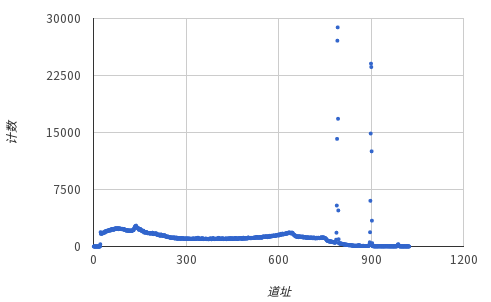
\includegraphics[width=0.45\textwidth]{1.png}
\\
\xiaowu\song 图~1\begin{minipage}[t]{75mm} \quad Co能谱图\\[-1mm]\wuhao
\end{minipage}
\end{center}

1.33MeV峰的计数为24058,对应的康普顿平台计数约为1131,所以峰康比为21.16。计算得到距今Co60的活度为2.5E5,1.33MeV峰下计数为87904个,测量活时为568s,所以计算可以得到相对探测效率为0.515。

接下来是利用Eu核素对探测器进行能量刻度, 具体的数据如下图:
\begin{center}
   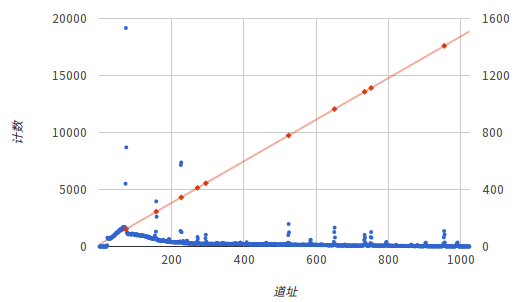
\includegraphics[width=0.45\textwidth]{2.png}
\\
\xiaowu\song 图~2\begin{minipage}[t]{75mm} \quad Eu能谱图以及标定曲线。\\[-1mm]\wuhao
\end{minipage}
\end{center}

从图中可以很清楚的看到Eu的各个能量峰,因而可以用他的具体数值进行标定。结果如下:

\begin{equation}
	E(KeV)=1.461*Channel +13.309
\end{equation}

同样的可以通过计算Eu源各个峰位的计数来得到相对探测效率曲线。如下图所示:
\begin{center}
   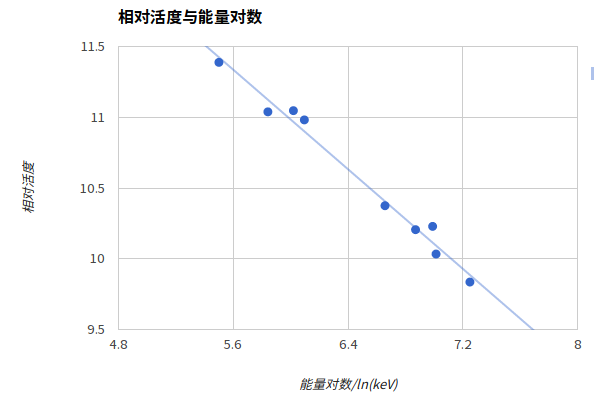
\includegraphics[width=0.45\textwidth]{3.png}
\\
\xiaowu\song 图~3\begin{minipage}[t]{75mm} \quad 相对探测效率曲线图。\\[-1mm]\wuhao
\end{minipage}
\end{center}

可以看出相对效率的对数于能量的的对数还是较为满足一个线性关系的。具体的值为:
\begin{equation}
	\ln(Relative Efficiency)=-0.879\times \ln(Energy)+16.26
\end{equation}

随后便是计算探测器的绝对探测效率。探测器在测量Co时候探测到的光子数目为87190个,实际发射的光子数目为$1.48\times 10^8$个,因而可以得到绝对探测效率为$6.1\times 10^{-4}$。将对应的数值替换即可得到各个能量对应的绝对探测效率,如下图所示:
\begin{center}
   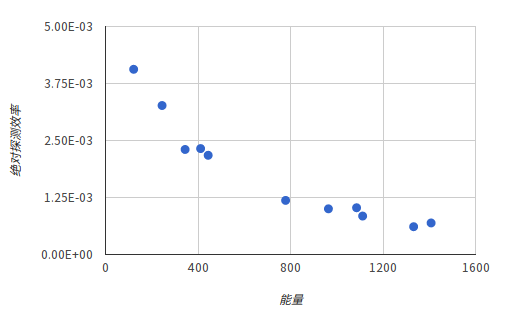
\includegraphics[width=0.45\textwidth]{4.png}
\\
\xiaowu\song 图~4\begin{minipage}[t]{75mm} \quad 绝对探测效率曲线图。\\[-1mm]\wuhao
\end{minipage}
\end{center}

分析混合源的能谱可以得到如下能谱图:

\begin{center}
   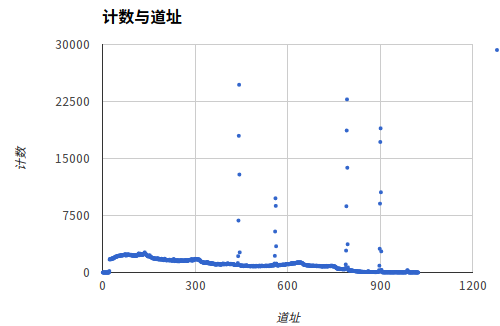
\includegraphics[width=0.45\textwidth]{5.png}
\\
\xiaowu\song 图~5\begin{minipage}[t]{75mm} \quad 混合源能谱图。\\[-1mm]\wuhao
\end{minipage}
\end{center}

从能谱中可以看出在443,561,792,902处有4个峰,根据之前的标定结果可以知道其对应的能量分别为660.5,834.4,1170.4,1331.1keV。分别是Cs137,Mn54,以及Co60的两个光电峰。

随后是对本底环境进行分析,改变放大器倍数为原来的两倍,从新利用Eu进行标定,标定结果如下:

\begin{center}
   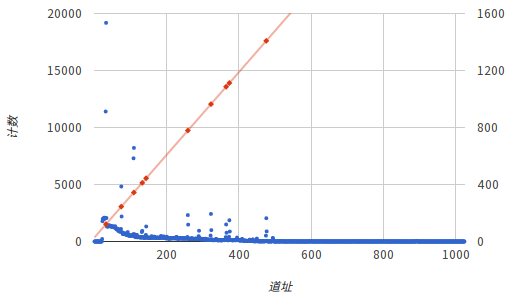
\includegraphics[width=0.45\textwidth]{6.png}
\\
\xiaowu\song 图~6\begin{minipage}[t]{75mm} \quad Eu新标定能谱图。\\[-1mm]\wuhao
\end{minipage}
\end{center}

\begin{equation}
	E(KeV)=2.904\times x +25.84
\end{equation}

从能谱图中可以根据各个峰位计算出对应的能量,从而得到本底中的各个辐射元素。本底能谱图计算的表格如下所示:

\begin{center}
   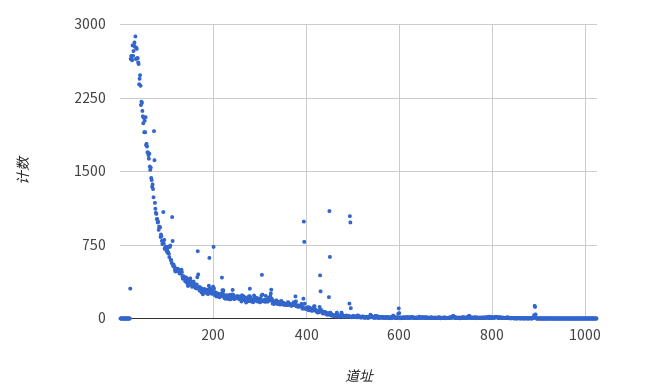
\includegraphics[width=0.45\textwidth]{7.png}
\\
\xiaowu\song 图~7\begin{minipage}[t]{75mm} \quad 背景辐射能谱图。\\[-1mm]\wuhao
\end{minipage}
\end{center}

\begin{center}
\bgliu
{\bf 表~1\quad
环境本地中的放射性元素测量表}\\[0.5mm]
\renewcommand{\arraystretch}{1.5}
\liuhao\song\rm
\newcolumntype{M}{>{\centering\arraybackslash}m{12mm} >{\centering\arraybackslash}m{12mm}>{\centering\arraybackslash}m{12mm}}
\begin{tabular}{M}
\specialrule{0.1em}{1pt}{1pt}

道址	&	能量/keV	&	对应核素	\\
\midrule
73	&	237.832	&	212Pb	\\
93	&	295.912	&	152Eu	\\
112	&	351.088	&	214Pb	\\
168	&	513.712	&	206Tl	\\
201	&	609.544	&	214Bi	\\
219	&	661.816	&	214Bi	\\
242	&	728.608	&	212Bi	\\
279	&	836.056	&	228Ac	\\
305	&	911.56	&	228Ac	\\
313	&	934.792	&	214Bi	\\
325	&	969.64	&	228Ac	\\
395	&	1172.92	&	60Co	\\
430	&	1274.56	&	22Na	\\
450	&	1332.64	&	60Co	\\
494	&	1460.416	&	40K	\\
599	&	1765.336	&	214Bi	\\
891	&	2613.304	&	208Tl	\\
\specialrule{0.1em}{3pt}{2pt}\\[-4mm]
\end{tabular}\\
\renewcommand{\arraystretch}{1.0}
\end{center}

\section{参考文献}

\noindent
[1] Peking Unviersity, Fudan University \ Nuclear Experment
\ Nuclear Publishing House, 1989 (in Chinese)

\noindent
 (北京大学,复旦大学.\ 原子核实验\ 原子能出版社,\ 1989)

\end{multicols}

\newpage

\clearpage
%\end{CJK*}
\end{document}

